\documentclass{standalone}
\usepackage{tikz}
\usetikzlibrary{shapes,arrows,positioning}
\begin{document}
  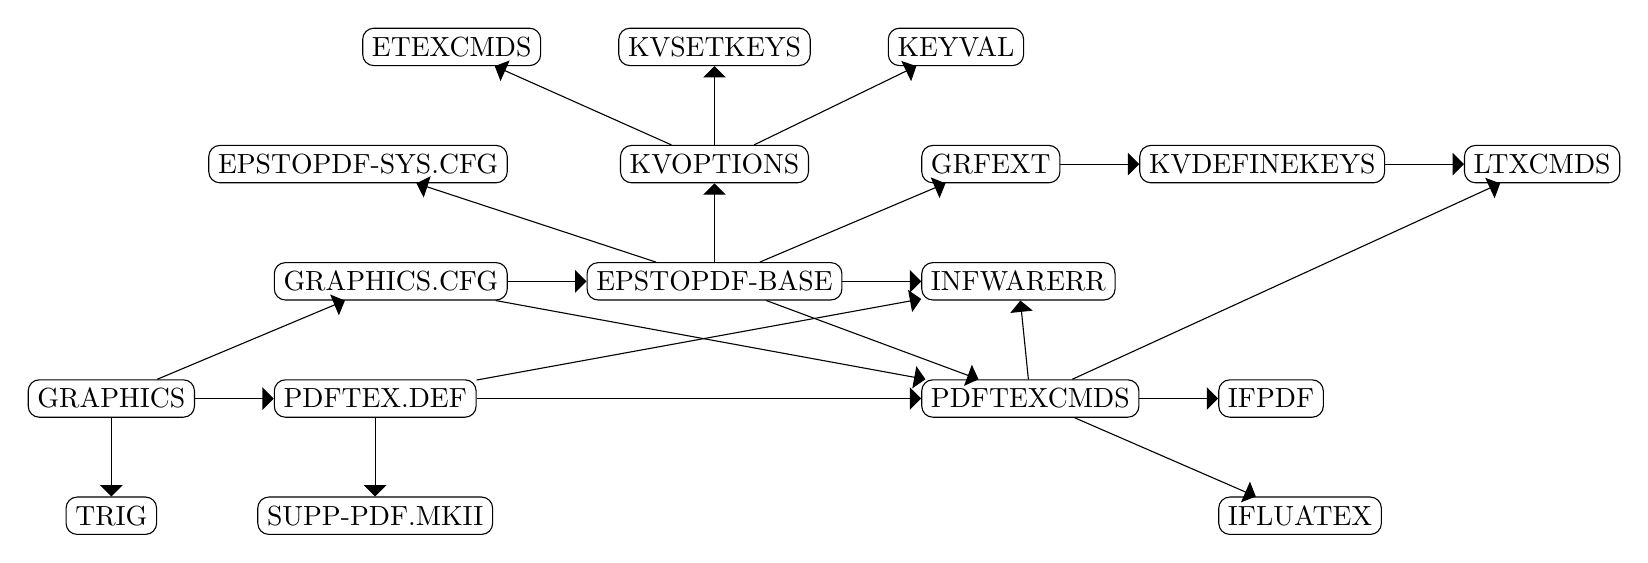
\begin{tikzpicture}
  
  \tikzset{main node/.style={rectangle, draw,
  		text centered, rounded corners}, }
  \tikzset{main verb/.style={minimum size=1cm}, }
  \tikzset{linea/.style={-triangle 90}, }
\node[main node] (a)   {GRAPHICS};
\node[main node] (b) [above right =of a]  {GRAPHICS.CFG};
\node[main node] (c) [right =of a]  {PDFTEX.DEF};
\node[main node] (d) [below =of a]  {TRIG};
\node[main node] (e) [below =of c]  {SUPP-PDF.MKII};



   
    \node[main node] (1)[right=of b]   {EPSTOPDF-BASE};
    %\node (2) [right =of 1]  {};
   \node[main node] (3) [ right =of 1]   {INFWARERR};
   \node[main node] (4) [above right =of 1] {GRFEXT};
   \node[main node] (5) [below right =of 1]  {PDFTEXCMDS};
   \node[main node] (6) [above =of 1] {KVOPTIONS};
   \node[main node] (7) [above right=of 6] {KEYVAL};
    \node[main node] (8) [above =of 6] {KVSETKEYS};
     \node[main node] (9) [above left=of 6] {ETEXCMDS};
\node[main node] (10) [right =of 4] {KVDEFINEKEYS};
\node[main node] (11) [right =of 10] {LTXCMDS};
 \node[main node] (12) [right =of 5]  {IFPDF};
 %\node[main node] (12) [above  =of 13]  {PDFTEXCMDS};
   \node[main node] (13) [below right =of 5]  {IFLUATEX};
   % \node[main node] (15) [below  =of 14]  {PDFTEXCMDS};
   
\node[main node] (f) [above left =of 1] {EPSTOPDF-SYS.CFG};   
   
 
\foreach \x /\y in{1/3,1/4,1/5,1/6,6/7,6/8,6/9,4/10,10/11,5/3,5/11,5/12,5/13,a/b,a/c,a/d,b/1,b/5,c/5,c/3,c/e,1/f}
  \path[linea] (\x) edge node {} (\y);
%%  
\end{tikzpicture}
\end{document}